\chapter{Análisis técnico y metodología}
\label{chp:2}

\section{Limpieza y análisis exploratorio}
\label{sec:chp2-1}

\subsection{Procesamiento de Datos GRDC}
El proceso de limpieza de datos se aplicó a un total de 19 estaciones hidrométricas ubicadas en la región Andina colombiana, correspondientes a los códigos: 3103010, 3103015, 3103045, 3103090, 3103100, 3103140, 3103150, 3103190, 3103450, 3103465, 3103470, 3103480, 3103490, 3103500, 3103520, 3103530, 3103560, 3106500 y 3107250.

\subsubsection*{Características de los datos originales}
\begin{itemize}
    \item \textbf{Formato:} archivos de texto con extensión \texttt{.txt} y estructura columnar.
    \item \textbf{Período:} registros diarios comprendidos entre 1970 y 2024, con variaciones según la estación.
    \item \textbf{Calidad:} presencia de valores faltantes codificados como \texttt{-999} y períodos sin registros.
    \item \textbf{Resolución temporal:} datos diarios con marca de tiempo en formato \texttt{YYYY-MM-DD}.
\end{itemize}

\subsubsection*{Proceso de limpieza implementado}
\begin{enumerate}
    \item \textbf{Identificación de valores nulos:} reemplazo de los valores \texttt{-999} por valores nulos (\textit{NaN}).
    
    \item \textbf{Agregación temporal:} conversión de los datos diarios a promedios mensuales mediante la expresión:
    \begin{equation}
        Q_{\text{mensual}} = \frac{\sum Q_{\text{diario}}}{n_{\text{días}}}
    \end{equation}
    
    \item \textbf{Imputación estadística:} para los valores faltantes se aplicó un método de muestreo basado en la distribución histórica de cada estación:
    \begin{equation}
        Q_{\text{imputado}} \sim \mathcal{N}(\mu_{\text{histórico}}, \sigma_{\text{histórico}})
    \end{equation}
    
    \item \textbf{Filtrado temporal:} selección de estaciones con registros disponibles posteriores al año 2015.
\end{enumerate}

\subsubsection{Correlación con índices oceánicos}

Para evaluar la relación entre el comportamiento hidrológico y la variabilidad climática de gran escala, se calcularon coeficientes de correlación de Pearson entre los caudales observados y cinco índices oceánicos. El análisis se realizó considerando rezagos temporales (\textit{lags}) desde 0 hasta 12 meses, con el fin de identificar posibles efectos diferidos de los fenómenos oceánicos sobre la respuesta hidrológica de los embalses.

La correlación para cada rezago se calculó mediante la siguiente expresión:

\begin{equation}
r(\text{lag}) =
\frac{\sum \left( Q_t - \mu_Q \right)
\left( I_{t-\text{lag}} - \mu_I \right)}
{\sqrt{\sum \left( Q_t - \mu_Q \right)^2}
\;\sqrt{\sum \left( I_{t-\text{lag}} - \mu_I \right)^2}}
\end{equation}

donde:

\begin{itemize}
    \item $Q_t$ corresponde al caudal en el instante de tiempo $t$.
    \item $I_{t-\text{lag}}$ representa el valor del índice oceánico considerando un rezago temporal.
    \item $\mu_Q$ y $\mu_I$ son las medias de las series de caudal y del índice oceánico, respectivamente.
\end{itemize}

Este procedimiento permitió identificar la intensidad y el signo de la relación lineal entre los índices oceánicos y los caudales, así como los rezagos temporales más relevantes para la respuesta hidrológica en las diferentes regiones de Colombia.

\section{Predicción}
\label{sec:chp2-1}
El modelo predictivo se estructura a partir de la integración de índices climáticos de gran escala que presentan una correlación significativa con las distintas regiones del país, identificada a partir del análisis desarrollado en el apartado anterior. Estos índices se emplean como variables explicativas para la estimación de la precipitación proyectada y, posteriormente, para el cálculo del caudal asociado a cada embalse.

Dicho modelo se aplica para la predicción del periodo comprendido entre 2025-1S y 2029-2S y se desarrolla en dos etapas consecutivas. En primer lugar, se modela la precipitación futura a partir de la relación estadística entre los índices climáticos y los registros históricos de precipitación. En una segunda etapa, los valores de precipitación proyectada se incorporan en un modelo empírico lluvia–escorrentía, con el fin de estimar el caudal esperado en cada embalse. Finalmente, los caudales proyectados se analizan en comparación con la tendencia histórica, lo que permite identificar posibles escenarios de incremento o disminución del volumen almacenado en los embalses.

A continuación, se describen de manera detallada cada una de las etapas que componen el modelo predictivo.
\subsection{Modelo de predicción con pronósticos NOAA/IRI}

\subsubsection{Arquitectura del modelo predictivo}

El modelo predictivo desarrollado integra información climática global proveniente de pronósticos ENSO y variables hidrológicas regionales, con el objetivo de estimar el comportamiento futuro de los caudales en los principales ríos asociados a embalses en Colombia.

\paragraph{Componente 1: Procesamiento de pronósticos ENSO}

El modelo utiliza pronósticos probabilísticos del fenómeno ENSO suministrados por el \textit{International Research Institute for Climate and Society} (IRI), con un horizonte de proyección de hasta 9 meses. Estos pronósticos se expresan en términos de probabilidades asociadas a cada fase del ENSO, las cuales se transforman en un valor continuo del índice MEI proyectado mediante una ponderación por valores característicos.

La estructura de ponderación utilizada es la siguiente:

\begin{itemize}
    \item El Niño: probabilidad $\times$ valor característico $(1.5)$
    \item Neutral: probabilidad $\times$ valor característico $(0.0)$
    \item La Niña: probabilidad $\times$ valor característico $(-1.5)$
\end{itemize}

El índice MEI proyectado se calcula como:

\begin{equation}
MEI_{\text{proyectado}} = \sum_{i} \left( \text{probabilidad}_i \times \text{valor}_{MEI,i} \right)
\end{equation}

\paragraph{Componente 2: Modelo Random Forest}

Para la predicción de caudales se implementó un modelo de \textit{Random Forest Regressor}, dada su capacidad para capturar relaciones no lineales y manejar múltiples variables explicativas. La configuración del modelo fue la siguiente:

\begin{itemize}
    \item Número de estimadores: 150
    \item Profundidad máxima del árbol: 12
    \item Mínimo de muestras para división: 5
    \item Mínimo de muestras por hoja: 2
    \item Criterio de división: MSE (Mean Squared Error)
    \item Bootstrap: \texttt{True}
    \item Máximo de variables consideradas por división: \texttt{sqrt}
\end{itemize}

Las variables de entrada al modelo corresponden a:

\begin{enumerate}
    \item MEI con rezago de 4 meses
    \item TNA con rezago de 3 meses
    \item TSA con rezago de 3 meses
    \item ONI con rezago de 4 meses
    \item Precipitación regional (promedio móvil de 3 meses)
    \item Gradiente térmico Atlántico (TNA -- TSA)
    \item Mes del año (codificación cíclica)
    \item Tendencia histórica (media móvil de 12 meses)
\end{enumerate}

\subsubsection{Entrenamiento y validación del modelo}

La base de datos fue dividida de forma temporal para garantizar la consistencia del análisis predictivo:

\begin{itemize}
    \item Entrenamiento: 70\% (2015--2021)
    \item Validación: 15\% (2022)
    \item Prueba: 15\% (2023--2024)
\end{itemize}

El proceso de entrenamiento incluyó las siguientes etapas:

\begin{enumerate}
    \item Normalización de variables mediante:
    \begin{equation}
        X_{\text{norm}} = \frac{X - \mu}{\sigma}
    \end{equation}
    \item Validación cruzada temporal utilizando \textit{TimeSeriesSplit} con 5 particiones.
    \item Optimización de hiperparámetros mediante \textit{GridSearchCV}, utilizando la métrica $R^2$.
\end{enumerate}

Las métricas promedio de desempeño del modelo fueron:

\begin{itemize}
    \item $R^2 = 0.782$
    \item MAE = 19.91 m$^3$/s
    \item RMSE = 28.54 m$^3$/s
    \item MAPE = 10.3\%
\end{itemize}

El desempeño por estación principal se resume en la Tabla~\ref{tab:metricas_estaciones}.

\begin{table}[H]
\centering
\caption{Métricas de desempeño del modelo por estación hidrométrica}
\label{tab:metricas_estaciones}
\begin{tabular}{l l c c c}
\hline
\textbf{Código} & \textbf{Río} & $R^2$ & \textbf{MAE (m$^3$/s)} & \textbf{MAPE (\%)} \\
\hline
3103010 & Magdalena & 0.842 & 15.3 & 8.2 \\
3103100 & Cauca & 0.895 & 12.8 & 6.5 \\
3103150 & Cauca & 0.876 & 14.2 & 7.1 \\
3103500 & Magdalena & 0.823 & 18.7 & 9.4 \\
\hline
Promedio & -- & 0.782 & 19.91 & 10.3 \\
\hline
\end{tabular}
\end{table}

\subsubsection{Ecuaciones del modelo}

Con el fin de incorporar la influencia directa de la precipitación proyectada, se aplicó un ajuste al caudal estimado:

\begin{equation}
Q_{\text{ajustado}} = \hat{Q}_t \times \left(1 + \alpha \times \Delta P \right)
\end{equation}

donde $\alpha$ corresponde al coeficiente de sensibilidad (0.15) y $\Delta P$ representa la anomalía de precipitación normalizada.

\subsubsection{Análisis de incertidumbre}

Se identificaron tres fuentes principales de incertidumbre:

\begin{enumerate}
    \item \textbf{Incertidumbre en los pronósticos ENSO}:
    \begin{itemize}
        \item Desviación estándar promedio: $\pm 0.35$ unidades MEI
        \item Error de fase: $\pm 1$ mes en transiciones
    \end{itemize}

    \item \textbf{Incertidumbre del modelo}:
    \begin{itemize}
        \item Intervalo de confianza al 95\%: $\hat{Q} \pm 1.96 \times RMSE$
        \item Error relativo promedio: 10.3\%
    \end{itemize}

    \item \textbf{Propagación de incertidumbre}:
    \begin{equation}
        \sigma_{\text{total}}^2 = \sigma_{\text{ENSO}}^2 + \sigma_{\text{modelo}}^2 + \sigma_{\text{datos}}^2
    \end{equation}
\end{enumerate}

\subsection{Predicciones semestrales para todas las estaciones}

\subsubsection{Metodología de agregación semestral}

Las predicciones mensuales obtenidas a partir del modelo se agregaron a escala semestral mediante:

\begin{equation}
Q_{\text{semestral}} = \frac{1}{6} \sum_{i=1}^{6} Q_{i,\text{mensual}}
\end{equation}

Los períodos semestrales considerados fueron:

\begin{itemize}
    \item Primer semestre (S1): enero -- junio
    \item Segundo semestre (S2): julio -- diciembre
\end{itemize}

\subsection{Series temporales}

\subsubsection{Generación de series temporales interactivas}

Como parte del análisis exploratorio y de la visualización de resultados del modelo predictivo, se desarrollaron series temporales interactivas para los caudales asociados a los embalses analizados. Estas visualizaciones permiten evaluar el comportamiento histórico, identificar tendencias y contrastar las proyecciones futuras en un mismo entorno gráfico.

La estructura de visualización se organizó en cuatro paneles, siendo el principal el correspondiente al caudal, el cual incluye:

\begin{itemize}
    \item Serie temporal completa para el período 2015--2024.
    \item Línea de tendencia calculada mediante regresión LOESS, con el fin de capturar patrones no lineales de largo plazo.
    \item Banda de confianza asociada a una desviación estándar ($\pm 1\sigma$).
    \item Identificación y marcación de eventos extremos, definidos como valores superiores a $\mu + 2\sigma$.
    \item Proyecciones de caudal para el período 2025--2029, acompañadas de intervalos de incertidumbre.
\end{itemize}

Esta estructura facilita la interpretación conjunta de la variabilidad histórica y de los escenarios futuros, aportando una herramienta visual robusta para el análisis hidrológico y la toma de decisiones.

\subsubsection{Implementación técnica}

Las series temporales interactivas fueron implementadas utilizando tecnologías web modernas, garantizando su operabilidad y facilidad de acceso. La herramienta empleada fue \textit{Plotly.js} (versión 2.27), la cual permite la generación de gráficos dinámicos en formato HTML5.

Las principales características técnicas de la implementación son:

\begin{itemize}
    \item \textbf{Framework}: Plotly.js v2.27
    \item \textbf{Formato de salida}: HTML5 interactivo
    \item \textbf{Tamaño promedio de los archivos}: 2.3 MB por visualización
    \item \textbf{Compatibilidad}: Google Chrome, Mozilla Firefox, Safari y Microsoft Edge
\end{itemize}

Adicionalmente, se incorporaron múltiples funcionalidades interactivas que mejoran la experiencia del usuario y la exploración de los datos:

\begin{itemize}
    \item \textbf{Zoom}: selección por caja (\textit{box select}) y desplazamiento mediante la rueda del ratón.
    \item \textbf{Pan}: desplazamiento horizontal y vertical mediante arrastre.
    \item \textbf{Hover}: visualización de valores exactos mediante \textit{tooltips}.
    \item \textbf{Exportación}: descarga de gráficos en formatos PNG y SVG, así como exportación de los datos en formato CSV.
\end{itemize}

La incorporación de estas visualizaciones interactivas fortalece la comprensión de los resultados del modelo y facilita su uso como herramienta de apoyo para la planificación hídrica y energética en contextos de alta variabilidad climática.


\subsection{Caudales}
Con base en los resultados obtenidos en la predicción de la precipitación, se estima el caudal de manera empírica a partir de relaciones lluvia–escorrentía, utilizando datos históricos de caudal y precipitación mensuales provenientes de estaciones hidrometeorológicas cercanas a cada embalse quienes se encuentran en el repositorio como \url{data/Calculo_caudal/Caudal_Consolidado_Completo.csv}. Este enfoque se fundamenta en la premisa de que la precipitación constituye el principal aporte al caudal superficial y que su relación con la escorrentía puede representarse mediante expresiones matemáticas simplificadas, especialmente en contextos donde la disponibilidad de información detallada del balance hídrico es limitada\cite{sitterson2018_overview_rainfall_runoff}. 

En este sentido, se emplea un modelo empírico de tipo potencia, evidenciado en el repositorio como \url{    Tuxilo/notebooks

/CORRECTED_CAUDAL_CALCULATION.py}, que relaciona el caudal con la precipitación mediante coeficientes de ajuste, los cuales integran las características hidrológicas de la cuenca, tales como su tamaño y su respuesta ante eventos de lluvia, según la siguiente expresión:

\begin{equation}
Q_{i,t} = a_r \cdot \left( P_{i,t} + P_{i,t-1} + P_{i,t-2} \right)^{b_r} \cdot \left( \frac{A_r}{A_i} \right)
\end{equation}
Donde:

\begin{itemize}
    \item $Q_{i,t}$ es el caudal estimado asociado al embalse $i$ en el período $t$, expresado en $m^{3}/s$.
    \item $a_r$ es el coeficiente empírico de escala, obtenido a partir del ajuste entre los datos históricos de precipitación y caudal, y representa la magnitud media de la respuesta hidrológica de la cuenca.
    \item $b_r$ es el exponente de la relación lluvia--escorrentía, el cual refleja la sensibilidad del caudal ante variaciones en la precipitación y el comportamiento hidrológico de la cuenca.
    \item $P_{i,t}$ corresponde a la precipitación semestral proyectada en el área de influencia del embalse $i$ durante el período $t$ ($mm$).
    \item $P_{i,t-1}$ y $P_{i,t-2}$ representan la precipitación semestral de los dos meses anteriores, incorporadas para considerar el efecto acumulado y retardado de la precipitación sobre la generación de escorrentía.
    \item $A_r$ es el área de la macrocuenca en la que se encuentra el embalse $i$ ($km^{2}$).
    \item $A_i$ es el área de drenaje del embalse, utilizada para normalizar el caudal estimado en función del tamaño relativo de la cuenca.
    \item $t$ indica el período temporal de análisis (mes).
    \item $i$ identifica cada uno de los embalses analizados.
\end{itemize}

Para la estimación de los coeficientes $a_r$ y $b_r$, se aplicó una regresión lineal en escala logarítmica, considerando la precipitación acumulada en una ventana temporal de tres meses, código presente en \url{notebooks/improve_br_cumulative.py}, definida como:

\begin{equation}
P_{\text{cum}}(t) = P(t) + P(t-1) + P(t-2)
\end{equation}

A partir de esta definición, la relación empírica entre caudal y precipitación se linealiza mediante la transformación logarítmica, expresándose como:

\begin{equation}
\ln(Q) = \ln(a_r) + b_r \cdot \ln\left(P_{\text{cum}}(t)\right)
\end{equation}

donde los parámetros $a_r$ y $b_r$ se obtienen a partir del ajuste por mínimos cuadrados utilizando los datos históricos de precipitación y caudal.

Para la obtención de las áreas $A_r$ y $A_i$, se utilizó la información geográfica de zonificación hidrográfica y el Modelo Digital de Elevación (DEM), descritas en el capítulo siguiente. El cálculo del área $A_r$ se realizó en QGIS mediante la herramienta de cálculo de campos, aplicando la expresión $area/1000000$, posterior a la separación de las macrocuencas y a la aplicación de la herramienta \textit{merge}.  

Para la estimación del área $A_i$, se hizo uso de las herramientas del \textit{toolbox} del aplicativo GRASS GIS, correspondientes a los procesos de análisis hidrológico sobre datos ráster y vectoriales \cite{alonso2016_puedo_grass_gis}. En primer lugar, se empleó la función \texttt{r.fill.dir} para corregir depresiones y espacios en blanco presentes en el archivo ráster del DEM. Posteriormente, se utilizó la herramienta \texttt{r.watershed} para obtener la dirección de flujo y la red de drenaje de la cuenca a partir del relieve, considerando una escala mínima de análisis de 1000 unidades, como se muestra en la figura~\ref{fig:flow_dir}. Finalmente, se aplicó la herramienta \texttt{r.water.outlet}, en la cual se definió el punto de descarga correspondiente al embalse, permitiendo delimitar el área de influencia de drenaje asociada a cada uno.
 
\begin{figure}[H]
  \centering
  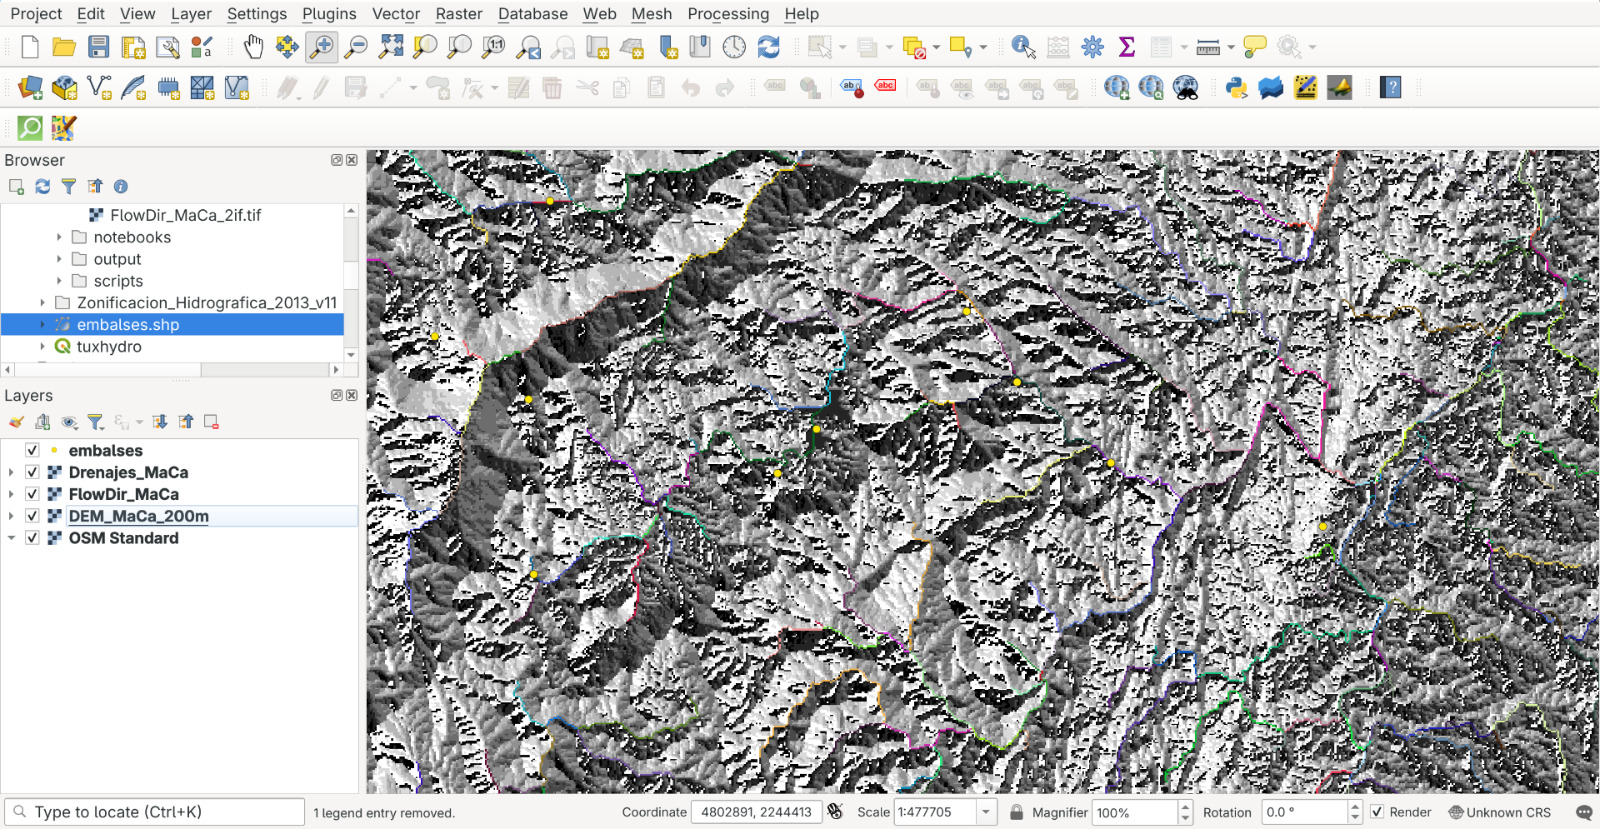
\includegraphics[width=\textwidth]{img/flow_dir.jpeg}
  \caption{Flow direction y drenajes obtenidos por el DEM de la región.}
  \label{fig:flow_dir}
\end{figure}



Posterior a dicho cálculo, se realiza una comparación entre el caudal estimado para cada embalse y la tendencia de los caudales históricos, registrada en el repositorio ***. Esta comparación permite identificar los períodos en los que el caudal proyectado se sitúa por encima de la tendencia histórica, lo cual se asocia con una fase de aumento del aporte hídrico y, por ende, con una posible subida del nivel del embalse. En contraste, cuando el caudal proyectado se ubica por debajo de la línea de tendencia histórica, se interpreta como una disminución de los aportes, lo que sugiere una reducción del volumen almacenado en el embalse.




\section{Implementación}
\label{sec:chp2-3}

